\documentclass[oneside]{modern}


%Deckblatt, falls nicht geht löschen :)

%  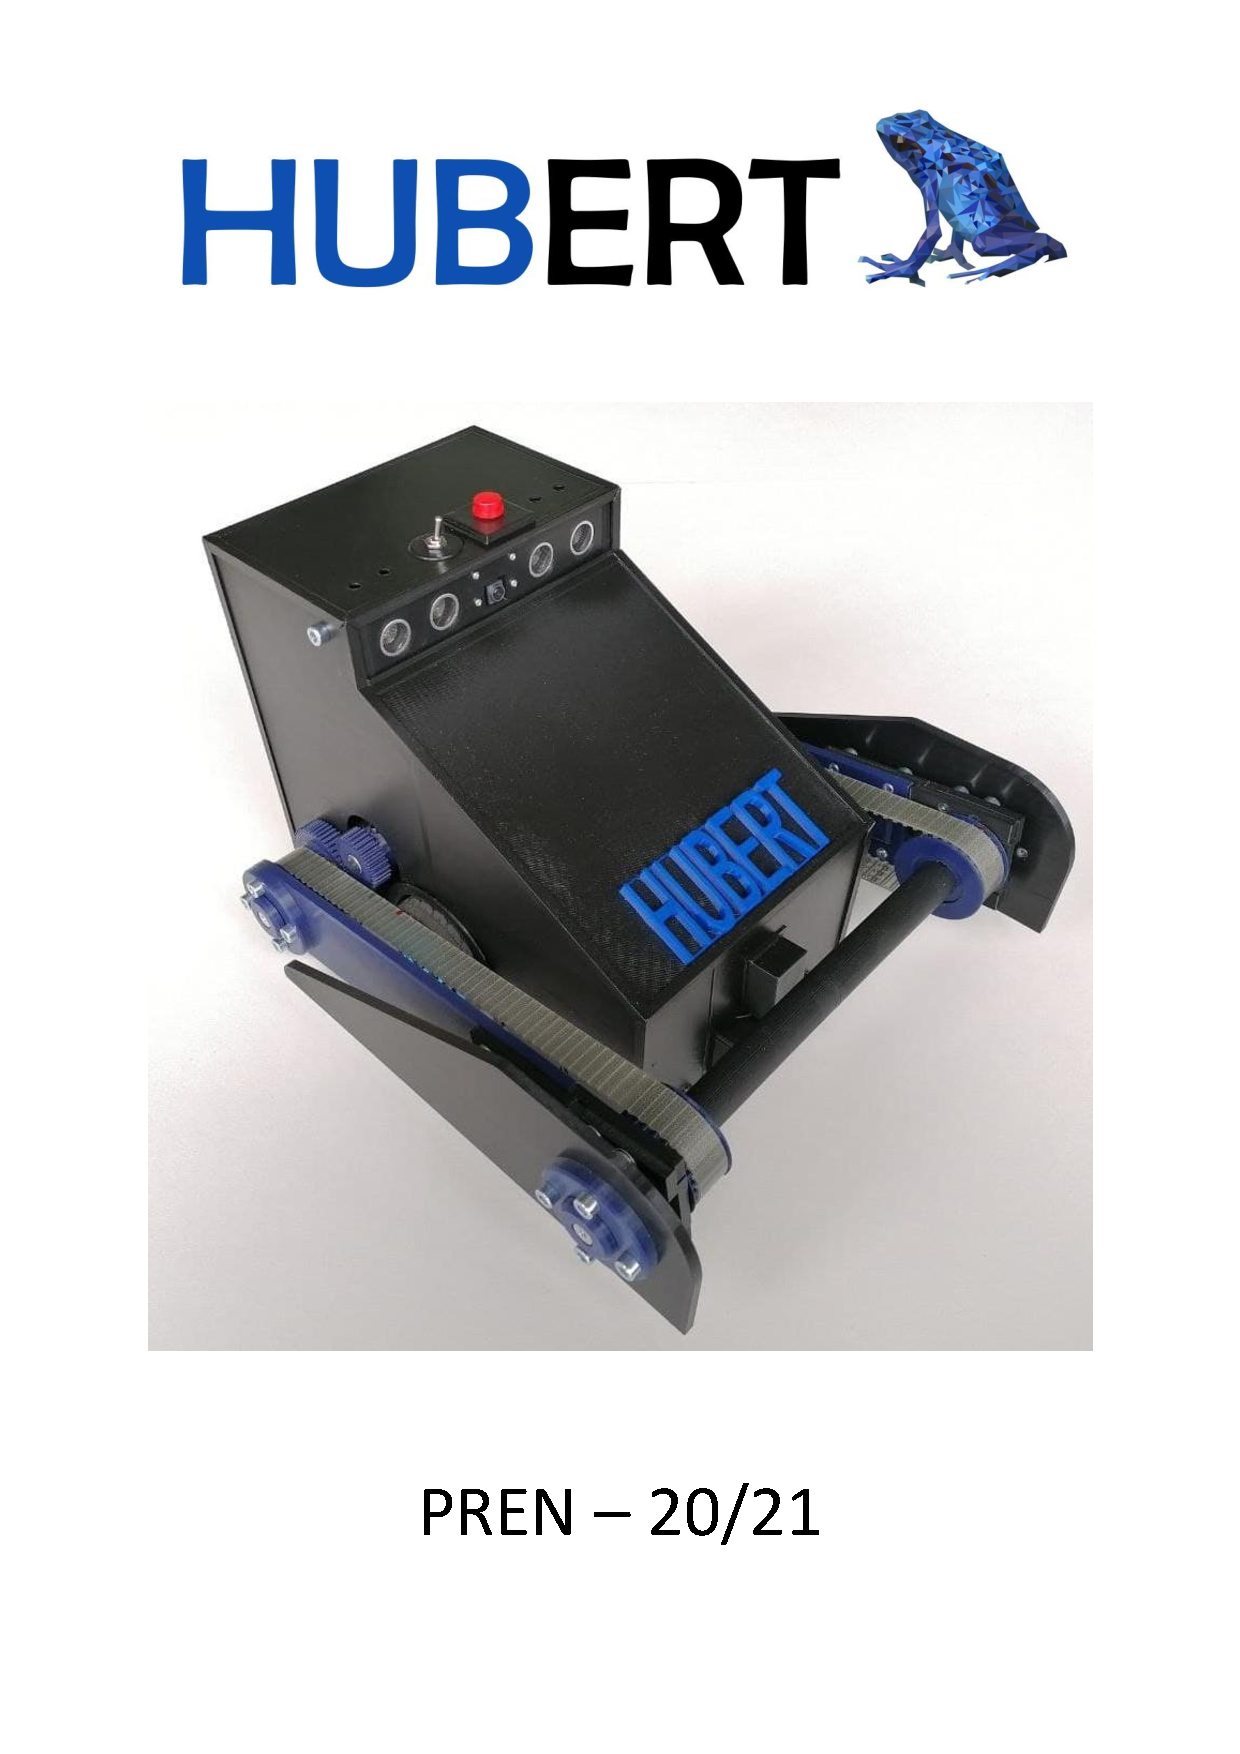
\includepdf[
 % pages={1-},
 % scale=0.9,
 % pagecommand={\pagestyle{fancy}}
%]{assets/Deckblatt.pdf}


\newpage


\title{Produktentwicklung 2}
\author{
\begin{tabular}{ l l l}
  \textbf{Gruppe 5} && \\
  Burch Sven & <sven.burch@stud.hslu.ch> & Maschinentechnik\\
  Burri Sven & <sven.burri@stud.hslu.ch> & Maschinentechnik \\
  Fassbind Benjamin & <benjamin.fassbind@stud.hslu.ch> & Informatik \\
  Jacob Yves & <yves.jacob@stud.hslu.ch> & Elektrotechnik\\
  Meier Boas & <boas.meier@stud.hslu.ch> & Informatik\\
  Roos Yannick & <yannick.roos@stud.hslu.ch> & Elektrotechnik \\
  \\
  \textbf{Betreuender Dozent} && \\
  Sollberger Peter & <peter.sollberger@hslu.ch> & Informatik \\
  \\
  \\
  \\
  TA.BA\_PREN2.F2101 &&\\
\end{tabular}
}


\newcommand{\sectionnumbering}[1]{%
  \setcounter{section}{0}%
   \renewcommand{\thesection}{\csname #1\endcsname{section}}}

\usepackage{etoc}
\etocsettocstyle
    {\section *{\contentsname
%                \@mkboth {\MakeUppercase \contentsname}
%                         {\MakeUppercase \contentsname}
         }
         }
    {}   
    
% ref packages
\usepackage{nameref}
% folowing  must be in this order
\usepackage{varioref}
\usepackage{hyperref}
\usepackage{cleveref}
\usepackage{url}

\begin{document}

   % magic * chapter starts at 1 :) 
   \renewcommand{\thesection}{\arabic{section}}
   % also break urls
   \makeatletter
   \g@addto@macro{\UrlBreaks}{\UrlOrds}
   \makeatother
   
   %\textcolor{light-gray}{\rule{\linewidth}{1pt}}

   %\PassOptionsToPackage{hyphens}{url}\usepackage{hyperref}

  % Print whole bibliographie
  \nocite{*}

  \firstpage
    {Autonomer Baugerüst-Roboter}
    {Hochschule Luzern - Technik und Architektur}
    {\theauthor}

  \subfile{parts/0-Redlichkeiterklärung.tex}
  \subfile{parts/0-Management_summary.tex}
  
  \newpage
  \etocdepthtag.toc{mtchapter}
  \etocsettagdepth{mtchapter}{subsection}
  \etocsettagdepth{mtappendix}{none}
  \addtableofcontents
  

  \newpage
  
  \subfile{glossary.tex}

  % ------------------------------------------------------------------------------
  % Assemble the document with the multiple parts
  
  \subfile{parts/0-doc-info}
  \subfile{parts/1-Einleitung}
  \subfile{parts/2-Aufgabenstellung}
  \subfile{parts/3-Hauptteil}
  \subfile{parts/3.0-VergleichFunktionsmuster}
  \subfile{parts/3.1-softwarearchitektur}
  \subfile{parts/3.2-piktogrammerkennung}
  \subfile{parts/3.3-hinderniserkennung.tex}
  \subfile{parts/3.4-embedded-linux-workflow.tex}
  \subfile{parts/4.1-Bedienungsanleitung}
  \subfile{parts/5-Vorgehen}
  \subfile{parts/6-schlussdiskussion}
  
    \newpage
  \listoffigures
  
  \newpage
  \listoftables


  \newpage
  \addglossary

  % Literaturverzeichnis
  \newpage
  \addcontentsline{toc}
    {section}
    {Literaturverzeichnis}

  \printbibliography[
    heading=subbibliography
  ]

  % Anhang
  \newpage
  \addcontentsline{toc}
    {section}
    {Anhang}
    
  \subfile{parts/anhang}

\end{document}